\section{System Architecture}
\label{sec:system_architecture}

\begin{figure*}[t]
    \centering
    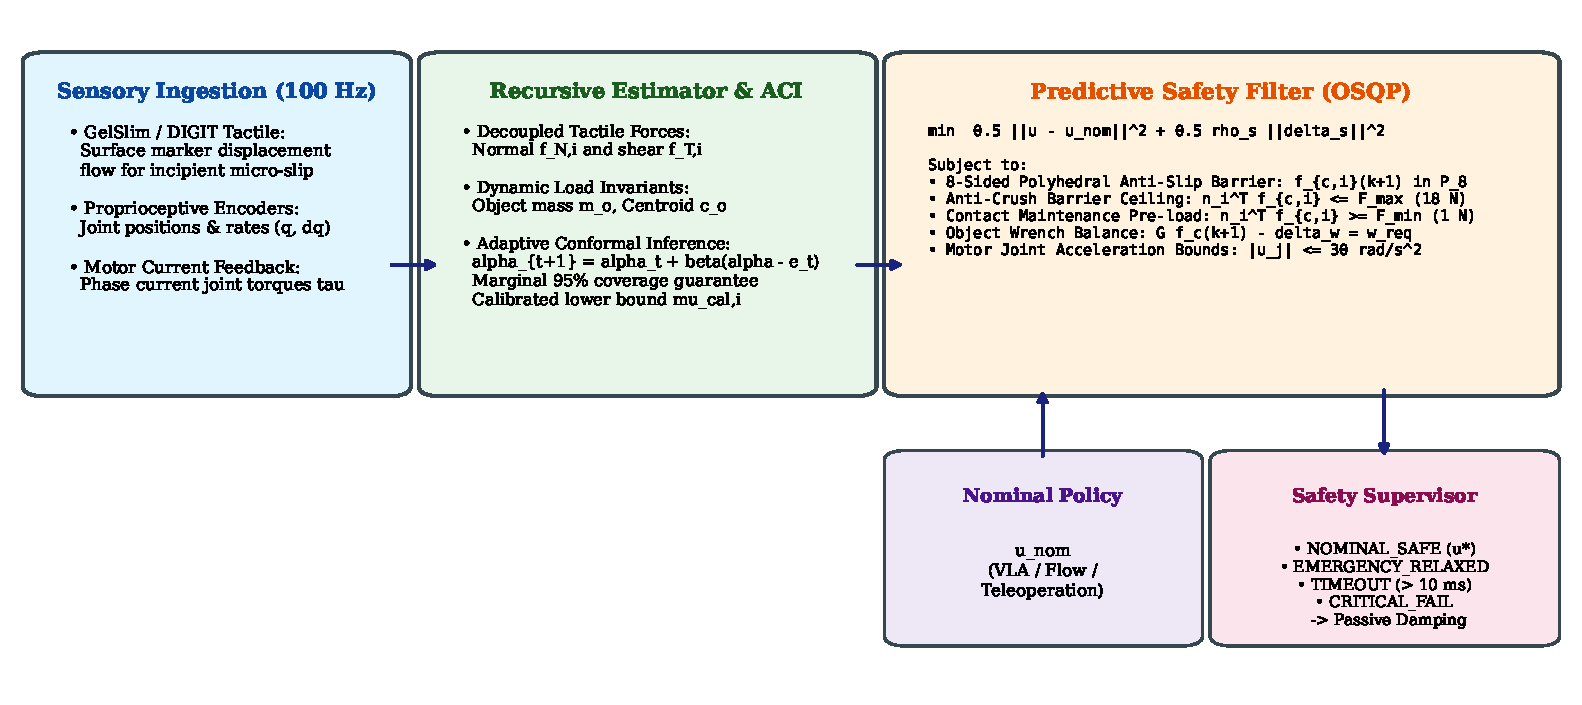
\includegraphics[width=\textwidth]{figures/architecture.pdf}
    \caption{\textbf{HOROS PROBE-1 End-to-End System Architecture.} High-speed sensory feedback ($100\text{ Hz}$ optical tactile marker flow, joint encoders, and motor effort) is processed by a multi-contact recursive estimator. The Adaptive Conformal Inference (ACI) module tracks non-exchangeable distribution shifts, supplying dynamically calibrated friction bounds $\mu_{\text{cal}, i}$ to the predictive safety filter. Operating at $100\text{ Hz}$, the OSQP Quadratic Program modifies nominal actions $\mathbf{u}_{\text{nom}}$ into certified safe joint accelerations $\mathbf{u}^*$, monitored by a real-time four-state decision gate.}
    \label{fig:architecture_overview}
\end{figure*}

The HOROS PROBE-1 architecture is designed as a modular, high-rate ($100\text{ Hz}$) predictive safety filter that intercepts nominal actions dispatched by upstream task planners (e.g., foundation VLA policies or human teleoperators) and projects them onto the certified safe contact set prior to actuation. As illustrated in \Cref{fig:architecture_overview}, the system comprises four interconnected functional tiers:

\subsection{Sensory Ingestion and Decoupled Contact Estimation}
At each $10\text{ ms}$ control cycle, the system ingests:
\begin{itemize}
    \item \textbf{Optical Tactile Afferents:} Elastomeric membrane deformation fields from four fingertip tactile sensors (GelSlim / DIGIT), parsed into local normal force $f_{N, i}$, tangential shear $\mathbf{f}_{T, i}$, and marker displacement field divergence for incipient slip detection.
    \item \textbf{Joint Encoders:} Articulated joint positions $\mathbf{q}_k \in \mathbb{R}^{16}$ and velocities $\dot{\mathbf{q}}_k \in \mathbb{R}^{16}$.
    \item \textbf{Actuator Effort:} Motor phase currents providing joint torque feedback $\boldsymbol{\tau}_k \in \mathbb{R}^{16}$.
\end{itemize}
These signals are processed by a recursive least-squares estimator tracking decoupled contact forces $\mathbf{f}_{c, i}(k)$, instantaneous object mass $\hat{m}_o(k)$, and Center of Mass $\hat{\mathbf{c}}_o(k)$.

\subsection{Non-Exchangeable Uncertainty Calibration Layer}
Rather than assuming nominal friction parameters, the estimation layer forwards raw contact residuals to an Adaptive Conformal Inference (ACI) module. Operating in closed-loop, ACI dynamically adjusts the empirical miscoverage quantile, outputting a certified lower friction bound $\mu_{\text{cal}, i}(k)$ that accounts for nonstationary distribution shifts without requiring unverified physical exchangeability.

\subsection{Predictive Safety Filter (QP Core)}
The core optimization engine constructs an action-dependent predictive Control Barrier Function (p-CBF) based on the linearized Hunt-Crossley sensitivity tensor $\mathbf{\Lambda}_i(\mathbf{q})$. The resulting convex Quadratic Program simultaneously enforces:
\begin{enumerate}
    \item 8-sided polyhedral anti-slip friction cone constraints ($\mathcal{P}_8$ inner polytope),
    \item Upper normal force crush limits to preserve fragile objects ($F_{\max} = 18.0\text{ N}$),
    \item Minimum contact maintenance thresholds ($F_{\min} = 1.0\text{ N}$),
    \item Object-level spatial wrench balance via the grasp matrix nullspace $\mathcal{N}(\mathbf{G})$, and
    \item Motor joint acceleration saturation limits ($|u_j| \le 30.0\text{ rad/s}^2$).
\end{enumerate}

\subsection{Real-Time Decision Gate and Fail-Safe Fallback}
A deterministic finite-state supervisor monitors solver convergence and watchdog latency. If the QP completes within the $10.0\text{ ms}$ budget with acceptable slack, the safe command $\mathbf{u}^*$ is dispatched directly to low-level motor torque controllers. If computational delays or physical infeasibility occur, the gate seamlessly transitions to passive damping fallback, guaranteeing failsafe dissipation of kinetic energy.
